%%%% Better Poster latex template example v1.0 (2019/04/04)
%%%% GNU General Public License v3.0
%%%% Rafael Bailo
%%%% https://github.com/rafaelbailo/betterposter-latex-template
%%%% 
%%%% Original design from Mike Morrison
%%%% https://twitter.com/mikemorrison

\documentclass[a0paper,fleqn]{betterposter}

%%%% Uncomment the following commands to customize the format

%% Setting the width of columns
% Left column
\setlength{\leftbarwidth}{0.27\paperwidth}
% Right column
\setlength{\rightbarwidth}{0.27\paperwidth}

%% Setting the column margins
% Horizontal margin
%\setlength{\columnmarginvertical}{0.05\paperheight}
% Vertical margin
%\setlength{\columnmarginhorizontal}{0.05\paperheight}
% Horizontal margin for the main column
%\setlength{\maincolumnmarginvertical}{0.15\paperheight}
% Vertical margin for the main column
%\setlength{\maincolumnmarginhorizontal}{0.15\paperheight}

%% Changing font sizes
% Text font
%\renewcommand{\fontsizestandard}{\fontsize{28}{35} \selectfont}
% Main column font
%\renewcommand{\fontsizemain}{\fontsize{28}{35} \selectfont}
% Title font
%\renewcommand{\fontsizetitle}{\fontsize{28}{35} \selectfont}
% Author font
%\renewcommand{\fontsizeauthor}{\fontsize{28}{35} \selectfont}
% Section font
%\renewcommand{\fontsizesection}{\fontsize{28}{35} \selectfont}

%% Changing font sizes for a specific text segment
% Place the text inside brackets:
% {\fontsize{28}{35} \selectfont Your text goes here}

%% Changing colours
% Background of side columns
%\renewcommand{\columnbackgroundcolor}{black}
% Font of side columns
%\renewcommand{\columnfontcolor}{gray}
% Background of main column
%\renewcommand{\maincolumnbackgroundcolor}{empirical}
%\renewcommand{\maincolumnbackgroundcolor}{theory}
%\renewcommand{\maincolumnbackgroundcolor}{methods}
%\renewcommand{\maincolumnbackgroundcolor}{intervention}
\renewcommand{\maincolumnbackgroundcolor}{lightgray}
% Font of main column
\renewcommand{\maincolumnfontcolor}{black}

\begin{document}    
\betterposter{
%%%%%%%% MAIN COLUMN

\maincolumn{
%%%% Main space

\textbf{Complete Vision!} 
%\newline
%\begin{center}
%    \noindent\begin{minipage}[b]{.455\textwidth}
%        \includegraphics[width=\linewidth]{img3}
%        \LARGE Light Interference$^{\text{2}}$
%    \end{minipage}%
%    \hfill
%    \begin{minipage}[b]{.4\linewidth}
%        \includegraphics[width=\linewidth]{img2}
%        \LARGE First holographic reconstruction, 1948$^{\text{2}}$
%    \end{minipage}
%    
%\end{center}
%
%\begin{center}
%\noindent\begin{minipage}[b]{.28\textwidth}
%    \includegraphics[width=\linewidth]{img0}
%    \LARGE Rasperry Pi camera as DHM sensor$^{\text{5}}$
%\end{minipage}%
%\hfill
%\begin{minipage}[b]{.44\linewidth}
%    \includegraphics[width=\linewidth]{img1}
%    \LARGE Holographic recosntruction of objects$^{\text{4}}$
%\end{minipage}


\begin{center}
	\noindent\begin{minipage}[b]{.5\textwidth}
		\includegraphics[width=0.7\linewidth, height=0.2\textheight]{img/img3}
		\newline
		\LARGE Light Interference$^{\text{2}}$
	\end{minipage}%
	\hfill
	\begin{minipage}[b]{.5\linewidth}
		\includegraphics[width=0.7\linewidth, height=0.2\textheight]{img/img2}
		\newline
		\LARGE First holographic reconstruction, 1948$^{\text{2}}$
	\end{minipage}
	
\end{center}

\begin{center}
	\noindent\begin{minipage}[b]{.5\textwidth}
		\includegraphics[width=0.6\linewidth, height=0.2\textheight]{img/img0}
		\newline
		\LARGE Rasperry Pi camera as DHM sensor$^{\text{5}}$
	\end{minipage}%
	\hfill
	\begin{minipage}[b]{.5\linewidth}
		\includegraphics[width=0.7\linewidth, height=0.2\textheight]{img/img1}
		\newline
		\LARGE Holographic reconstruction of objects$^{\text{4}}$
	\end{minipage}

\end{center}
}{
%%%% Bottom space
%% QR code
\qrcode{img/frame}{img/smartphoneWhite}{
\textbf{Take a picture} to
\\visit the project page
}
% Smartphone icon
% Author: Freepik
% Retrieved from: https://www.flaticon.com/free-icon/smartphone_65680

%% Compact QR code (comment the previous command and uncomment this one to switch)
%\compactqrcode{img/qrcode}{
%\textbf{Take a picture} to
%\\download the full paper
%}

}

}{
%%%%%%%% LEFT COLUMN

\title{Digital Holographic \\ Microscopy and Python }
\author{Nishadh K.A}
%\author{Rafael Bailo}
%\institution{Optional Institution Under Name}

\section{Introduction}


\begin{itemize}
    
    
    \item Holograms are Interference, circular pattern of bright and dark lines surrounding an object due to light \\passage over it in 2D plane$^{\text{1}}$.
    
    \item Holograms contains both light intensity and phase/field; in comparison, a photograph contains only intensity. So more information$^{\text{2}}$.
    
    \item  The Hungarian-British physicist Dennis Gabor was awarded Nobel Prize for inventing and applying this phenomenon for improving electron microscopy in 1971.
    
    \item Digital Holographic Microscopy (DHM) employes numerical reconstruction models/algorithms to visualise image; here computation acts as lens$^{\text{3}}$.
    
\end{itemize}

\section{Holopy}

\begin{itemize}
\item Conventionally, holograms are reconstructed, bypassing the light through holograms recorded in film plates. In DHM, there is a method of using backpropagation algorithms to reconstruct image$^{\text{4}}$.

\item There is an inference method that uses scattering models to simulate light scattering and an algorithm iteratively to match the recorded hologram to simulation.

\item Holopy$^{\text{1}}$, a Python library uses the inference method, which avoids inherent drawbacks of the backpropagation algorithm, such as the inclusion of non-physical interactions in the analysis.

\item The library uses legacy scattering models written in \\ Fortran.

\end{itemize}



%\begin{center}
%% Linear regression
%% Author: Henri Menke
%% Retrieved from: http://www.texample.net/tikz/examples/linear-regression/
%\includegraphics[width=\textwidth]{img/tikzexample1}
%\end{center}

%\section{Fundamental Theorem\\of Calculus}
%If $f$ is continuous on the closed interval $[a,b]$ and $F$ is the indefinite integral of $f$ on $[a,b]$, then
%\begin{equation}
%\int_a^b f(x)\,\mathrm{d}x = F(b)-F(a).
%\end{equation}
%
%\section{Conclusion}
%This is a great poster format!
%
%%% This fills the space between the content and the logo
%\vfill
%
%%% Institution logo
%%\includegraphics[width=\textwidth]{img/logo}\\

}{
%%%%%%%% RIGHT COLUMN

\section{Extended Role of Python}

\begin{itemize}
\item Major advantage of DHM is its application in light microscopy context, replacing expensive Laser and lens with numerical computations$^{\text{3}}$. 

\item The sensors are Complementary Metal-Oxide Semiconductors (CMOS)$^{\text{4}}$, a regular mobile phone camera without a lens and other optical components. LED works as light source. Making the hardware setup low cost. 

\item DHM gives insight into size and structure of the object being imaged, its 3-Dimensional information, topography along with autofocus feature$^{\text{3}}$. 

\item Robustness of holography in the noisy environment makes a suitable solution in environmental monitoring$^{\text{3}}$.

\item A recent study has shown the application of it in air pollution monitoring. Detection of Particulate Matter (PM) with accurate particle sizing, shape, and type. The study also used machine learning techniques in various processing steps in holography reconstruction$^{\text{4}}$.   

\item Python with the extensive ecosystem in machine learning and computer vision makes a vital tool in digital holographic/computational microscopy$^{\text{1}}$. 

\end{itemize}

\section{References}

1. Barkley, Solomon, et al. "Holographic microscopy with Python and HoloPy." Computing in Science and Engineering (2019).

2. Gabor, Dennis. "Holography, 1948–1971, Nobel Lecture." Imperial Colleges of Science and Technology.

3. Wikipedia contributors. "Digital holographic microscopy." Wikipedia, The Free Encyclopedia. Wikipedia, The Free Encyclopedia, 28 Sep. 2019. 

4. Wu, Yi-Chen, et al. "Air quality monitoring using mobile microscopy and machine learning." Light: Science \& Applications 6.9 (2017): e17046.

5. Werner, Kleindienst, et al. "Digital Inline Holographic Microscopy - An iGEM Approach." http://2017.igem.org/Team:TU, 10 Oct. 2019. 
%5. Wu, Yichen, et al. "Spatial mapping and analysis of aerosols during a forest fire using computational mobile microscopy." Optics and Biophotonics in Low-Resource Settings IV. Vol. 10485. International Society for Optics and Photonics, 2018.


\section{Acknowledgements}
\setlength{\maincolumnmarginhorizontal}{0.1\paperheight}
{\fontsize{23}{35} \selectfont The poster template is based on Betterposter-Latex \\ https://github.com/rafaelbailo/betterposter-latex-template}
    


}
\end{document}
